\chaptertitlepage{The Italian Typology}{Five archetypes of late-life experience in Italy}
\label{ch:ch4}

\section{Overview}
\label{sec:ch4-overview}

This chapter presents the five-archetype typology of the Italian over-65 population recovered from the K-means segmentation of Chapter~3. \S\ref{sec:ch4-five-archetypes} reports the population-level structure of the partition. \S\ref{sec:ch4-profile-descriptions} describes the five archetypes profile by profile. \S\ref{sec:ch4-integrative-view} presents the integrative profile fingerprint. \S\ref{sec:ch4-external-validation} reports external validation against life satisfaction. \S\ref{sec:ch4-demographics} reports the demographic composition by gender and age band. \S\ref{sec:ch4-isolation-paradox} develops the Isolation Paradox --- the most distinctive and policy-relevant finding of the Italian typology. \S\ref{sec:ch4-synthesis} closes with synthesis.

All centroid coordinates are reported as z-scores within Italy on the analytical sample ($n = 2{,}378$). The substantive direction of each variable is reported in parenthesis at first mention. National projection uses the Istat 2024 estimate of 14.18 million Italian residents aged 65 or older.

\section{The five archetypes}
\label{sec:ch4-five-archetypes}

The K-means segmentation with $k = 5$ partitions the 2,378 Italian respondents into five clusters. Figure~\ref{fig:ch4-profiles} reports cluster mean values on eight diagnostic variables, with profiles ordered from most fragile (left) to most connected (right). Table~\ref{tab:ch4-archetypes} lists the archetypes with their headline signature and population shares.

\begin{figure}[ht]
  \centering
  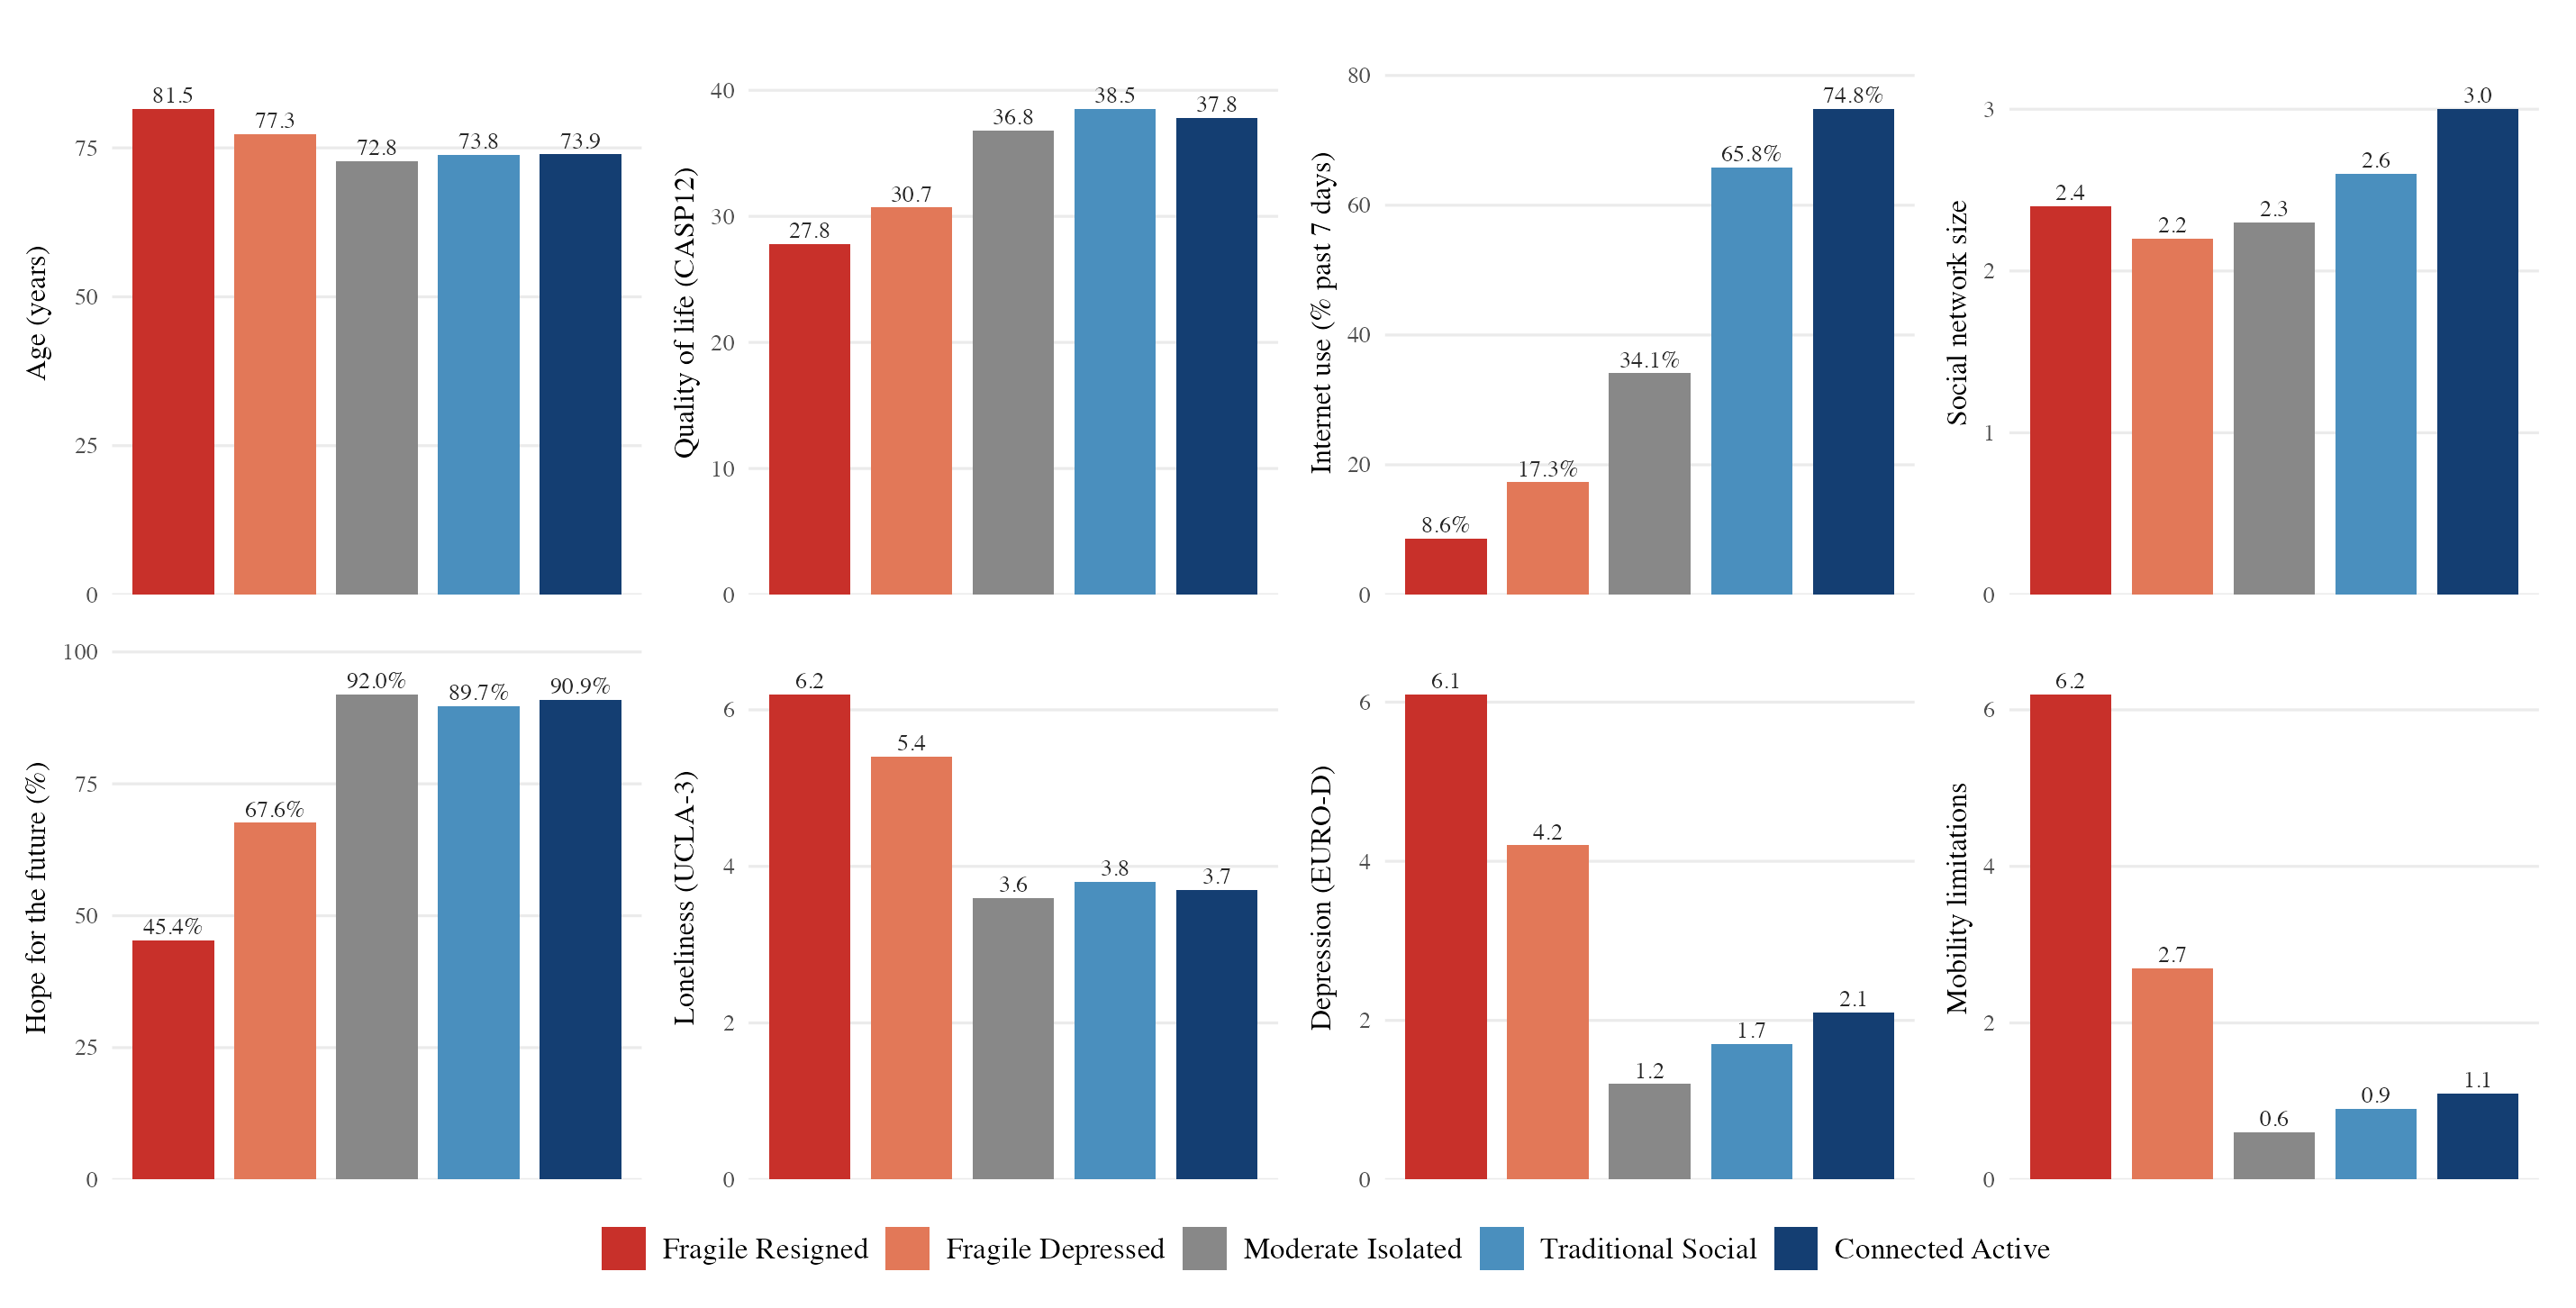
\includegraphics[width=0.95\linewidth]{figures/04_italy/fig_4_1_NEW.png}
  \caption{Profile characteristics, Italy. Mean values for each of the five archetypes on eight key dimensions: age, CASP-12 (12--48), internet (\% in past seven days), loneliness (UCLA-3, higher = lonelier), hope for the future (\% reporting hopes), social-network size, EURO-D depression (higher = more depressive symptoms), mobility limitations. Profiles ordered from most fragile to most connected. $N = 2{,}378$.}
  \label{fig:ch4-profiles}
\end{figure}

\begin{table}[ht]
  \centering
  \caption{Headline signature of the five Italian archetypes}
  \label{tab:ch4-archetypes}
  \begin{tabular}{p{2.5cm}p{1.2cm}p{7cm}}
    \toprule
    \textbf{Archetype} & \textbf{Share} & \textbf{Headline signature} \\
    \midrule
    Fragile Resigned & 14.4\% & Worst health, oldest age (mean 81.5 yr), lowest internet use (8.6\%) and CASP (27.8). Sub-clinical depression (EURO-D 6.1). Withdrawn evaluative orientation (hope 45.4\%). \\
    Fragile Depressed & 11.7\% & Persistent depressive affect (EURO-D 4.2, loneliness 5.4) with intermediate functional health and below-average resources. \\
    Moderate Isolated & 28.1\% & Average to good health (mobility 0.6, EURO-D 1.2) and resources, but restricted social engagement (network 2.3, internet 34.1\%). The largest single archetype and the country-specific Italian configuration. \\
    Traditional Social & 25.1\% & Good health and resources, dense cultural participation (hope 89.7\%), moderate internet adoption (65.8\%). Highest CASP (38.5). \\
    Connected Active & 20.7\% & Highest digital adoption (74.8\%), largest network (3.0), best resources, intact health. CASP 37.8. The silver-economy frontier of the Italian over-65 population. \\
    \bottomrule
  \end{tabular}
\end{table}

\noindent\small Note. Headline values are raw means of the diagnostic variables of Figure~\ref{fig:ch4-profiles}. Standardised centroid coordinates are reported in \S\ref{sec:ch4-profile-descriptions}. \normalsize

Two raw-scale observations from Figure~\ref{fig:ch4-profiles} anchor the standardised description that follows. First, the age gradient: the Fragile Resigned cluster has a mean age of 81.5 years, against 77.3 (Fragile Depressed), 72.8 (Moderate Isolated), 73.8 (Traditional Social) and 73.9 (Connected Active). The Fragile Resigned are on average eight years older than the four other archetypes, identifying the oldest-old segment of the population. Second, the digital divide: 8.6\% in Fragile Resigned versus 74.8\% in Connected Active --- a near nine-fold gap on a single behavioural indicator. From the silver-economy perspective, this gap defines the boundary between sub-populations served by digital products and those for whom traditional welfare and family-based provision remain the only operational channel.

\section{Profile descriptions}
\label{sec:ch4-profile-descriptions}

\subsection{Fragile Resigned}
\label{sec:ch4-fragile-resigned}

The Fragile Resigned cluster accounts for 14.4\% of the Italian over-65 population ($\approx 2.04$ million individuals). It sits at the most adverse end of every health dimension: self-rated health $+1.06$ (higher = worse), IADL $+1.97$, mobility $+1.38$, ADL $+1.74$, chronic conditions $+0.85$, EURO-D $+1.04$, physical inactivity $+1.05$. Mean age is 81.5 years --- eight years above the typology average --- identifying the oldest-old segment. Economic resources are below the Italian mean (log\_thinc $-0.19$, log\_hnetw $-0.34$) but the gap is small in standardised terms; the principal axis of fragility is health and functional autonomy, not income.

The subjective signature is the lowest in the typology on every evaluative dimension. CASP-12 is at $-1.02$ (raw 27.8), hope for the future at $-0.82$ (45.4\% report hopes, against $\geq 90\%$ in non-fragile profiles), interest at $-0.50$, expected survival at $-0.59$, loneliness at $+0.88$. The combination --- high subjective burden, low evaluative function, low expectation --- supports the descriptive label ``Resigned'': a cluster evaluatively withdrawn, with a configuration consistent with chronic adaptation to the constraints of advanced old age. Cognitive deficits are pronounced (orienti $-1.00$, fluency $-0.75$). The cluster is the principal target of the Italian long-term-care welfare branch and identifies the lower bound of the silver-economy market: a sub-population whose digital and behavioural channels are essentially closed and whose service consumption is mediated by family caregivers and institutional providers \citep{ferrera1996, saraceno2010}.

\subsection{Fragile Depressed}
\label{sec:ch4-fragile-depressed}

The Fragile Depressed cluster accounts for 11.7\% ($\approx 1.66$ million). It is intermediate on objective health and functional dimensions (sphus $+0.47$, EURO-D $+0.54$ with raw mean 4.2 just above the four-point clinical threshold, mobility $+0.36$, chronic conditions $+0.32$). Mean age is 77.3 years. Economic resources are below the Italian mean (log\_thinc $-0.39$, log\_hnetw $-0.40$, fdistress $-0.51$). The subjective signature is the second-lowest in the typology but qualitatively different from Fragile Resigned: CASP $-0.67$ (raw 30.7), loneliness $+0.59$ (raw 5.4), hope $-0.28$ (67.6\% report hopes --- clearly above 45.4\% of Fragile Resigned but below the non-fragile profiles). The cluster displays elevated depressive affect and loneliness without the same magnitude of withdrawal from hope and interest --- an active depressive episode rather than a settled withdrawal.

The contrast with Fragile Resigned is among the most substantively important findings of the Italian typology and one of the principal arguments for retaining $k = 5$ over $k = 4$ (Chapter~3). Demographically, the cluster is over-represented among Italian women: 31\% of women fall in Fragile Depressed against 22\% of men (\S\ref{sec:ch4-demographics}). Internet use is 17.3\% --- non-trivial but well below the non-fragile profiles. From the silver-economy perspective, the Fragile Depressed represent a configuration in which behavioural and digital channels remain partially open but the affective barrier is the binding constraint on adoption.

\subsection{Moderate Isolated}
\label{sec:ch4-moderate-isolated}

The Moderate Isolated cluster is the largest, at 28.1\% of the over-65 population ($\approx 3.98$ million individuals). The cluster sits at or near the Italian mean on most objective health and resource dimensions: sphus $-0.58$ (better than mean), EURO-D $-0.68$ (raw 1.2, well below the clinical threshold), mobility $-0.61$, IADL $-0.42$, log\_thinc $-0.33$, log\_hnetw $-0.22$, fdistress $-0.16$. Mean age is 72.8 years (the youngest of the five archetypes). The cluster is not characterised by adversity on health or economic dimensions: it is, in absolute terms, an averagely-resourced and averagely-healthy segment.

The diagnostic feature is the position on social, cultural and digital dimensions: network size $-0.22$ (raw 2.3 confidants), social\_integration $-0.11$, internet $-0.11$ (raw 34.1\%), three cultural-engagement indicators between $-0.15$ and $-0.37$, provision of help to grandchildren $-0.15$. None of these distances is large in absolute terms, but the joint pattern across the social and cultural variables identifies a configuration in which the social and informational ecosystem is materially thinner than in the rest of the typology. The cluster does not report itself as particularly lonely (loneliness raw 3.6, well below the Italian mean), despite the thin network --- consistent with the observation that loneliness in older age is less a function of absolute network size than of the discrepancy between desired and actual configuration \citep{hawkleycacioppo2010}.

The Moderate Isolated archetype is the most distinctive feature of the Italian typology and does not have a structural counterpart in the Swedish typology of Chapter~5. The substantive interpretation, developed in Chapter~6, is that this configuration reflects the Mediterranean familistic regime: a substantial fraction of the Italian middle stratum is socially anchored to the immediate family and the residential neighbourhood, with limited participation in the kinds of associational and cultural activities that the Swedish welfare state and civil society make available to comparable individuals. The behavioural and policy consequences --- including the under-utilisation of healthcare relative to Traditional Social peers --- are developed in \S\ref{sec:ch4-isolation-paradox} as the Isolation Paradox.

\subsection{Traditional Social}
\label{sec:ch4-traditional-social}

The Traditional Social cluster accounts for 25.1\% ($\approx 3.56$ million). It sits in the upper region of the resource and health distributions (sphus $-0.40$, IADL $-0.42$, log\_thinc $+0.41$, log\_hnetw $+0.55$, fdistress $+0.43$; mean age 73.8 years), in a comparable position to the Connected Active. The diagnostic feature is the configuration of social, cultural and digital engagement: the centroid is at $+3.29$ standard deviations on the cultural-engagement indicator ac035d5, $+0.43$ on ac035d1, $+0.50$ on educational participation (ac035d8), $+0.50$ on provision of help to grandchildren (sp008\_), $+0.62$ on social integration. Internet use is at $+0.53$ (raw 65.8\%) --- well above the Italian mean but materially below Connected Active (74.8\%).

The cluster is the carrier of a dense and traditional pattern of social and cultural participation: institutionalised cultural attendance, organised volunteering, intergenerational support, and a moderate digital engagement that complements rather than substitutes for offline activities. CASP-12 is the highest in the typology (raw 38.5, $z = +0.66$), loneliness is low ($z = -0.39$), hope is positive (89.7\%). From the silver-economy perspective, the cluster is the segment most receptive to hybrid product designs that combine digital interfaces with offline community channels (parish-based or club-based intermediation of digital services), while the Connected Active cluster supports direct-to-consumer digital products without intermediation.

\subsection{Connected Active}
\label{sec:ch4-connected-active}

The Connected Active cluster accounts for 20.7\% ($\approx 2.94$ million). It sits at the high-resource end of the typology on every economic dimension (log\_thinc $+0.72$, log\_hnetw $+0.64$, ypen1 $+0.53$, home\_own $+0.24$, fdistress $+0.68$) and on every health dimension (sphus $-0.28$, EURO-D $-0.25$, mobility $-0.30$, chronic $-0.12$). Mean age is 73.9 years. The diagnostic feature is digital integration and informational engagement: internet use at $+0.72$ (raw 74.8\%, the highest in the Italian typology), educational participation at $+0.74$, verbal fluency at $+0.63$ (the highest cognitive score), network size at $+0.42$ (raw 3.0, the highest). The configuration is the ``successful aging'' pattern of the gerontological literature \citep{rowekahn1997} operationalised on a contemporary Italian sample. CASP-12 is high (raw 37.8, $z = +0.56$), loneliness is low (raw 3.7), hope is at 90.9\%, expected survival at $+0.18$.

The Connected Active cluster maps onto the Swedish Connected Wealthy archetype with broadly similar standardised positions, but represents a smaller share (20.7\% vs 29.5\% in Sweden (Connected Wealthy archetype) --- Chapter~6). From the silver-economy perspective, the cluster constitutes the immediate and ready-to-serve market for digital products and services targeted at older adults in Italy: 2.94 million individuals with high digital adoption, high economic resources, and intact health. Together with Traditional Social (3.56 million, partially digitally engaged), the Connected Active cluster defines the upper bound of the Italian silver-economy addressable market under current technology-adoption conditions.

\section{Integrative view: the typology fingerprint}
\label{sec:ch4-integrative-view}

The five-archetype centroid configuration is visualised in two complementary forms. Figure~\ref{fig:ch4-fingerprint} reports the profile fingerprint as a faceted view, with one panel per archetype showing the standardised mean across the 29 active variables; variables are grouped by dominant Factor Analysis loading (Chapter~3). Figure~\ref{fig:ch4-fa-scatter} plots all Italian respondents on the FA1 $\times$ FA2 plane (FA1: physical and functional fragility; FA2: high values correspond to worse subjective wellbeing), with diamonds marking cluster centroids and ellipses marking 50\% confidence regions per profile.

\begin{figure}[ht]
  \centering
  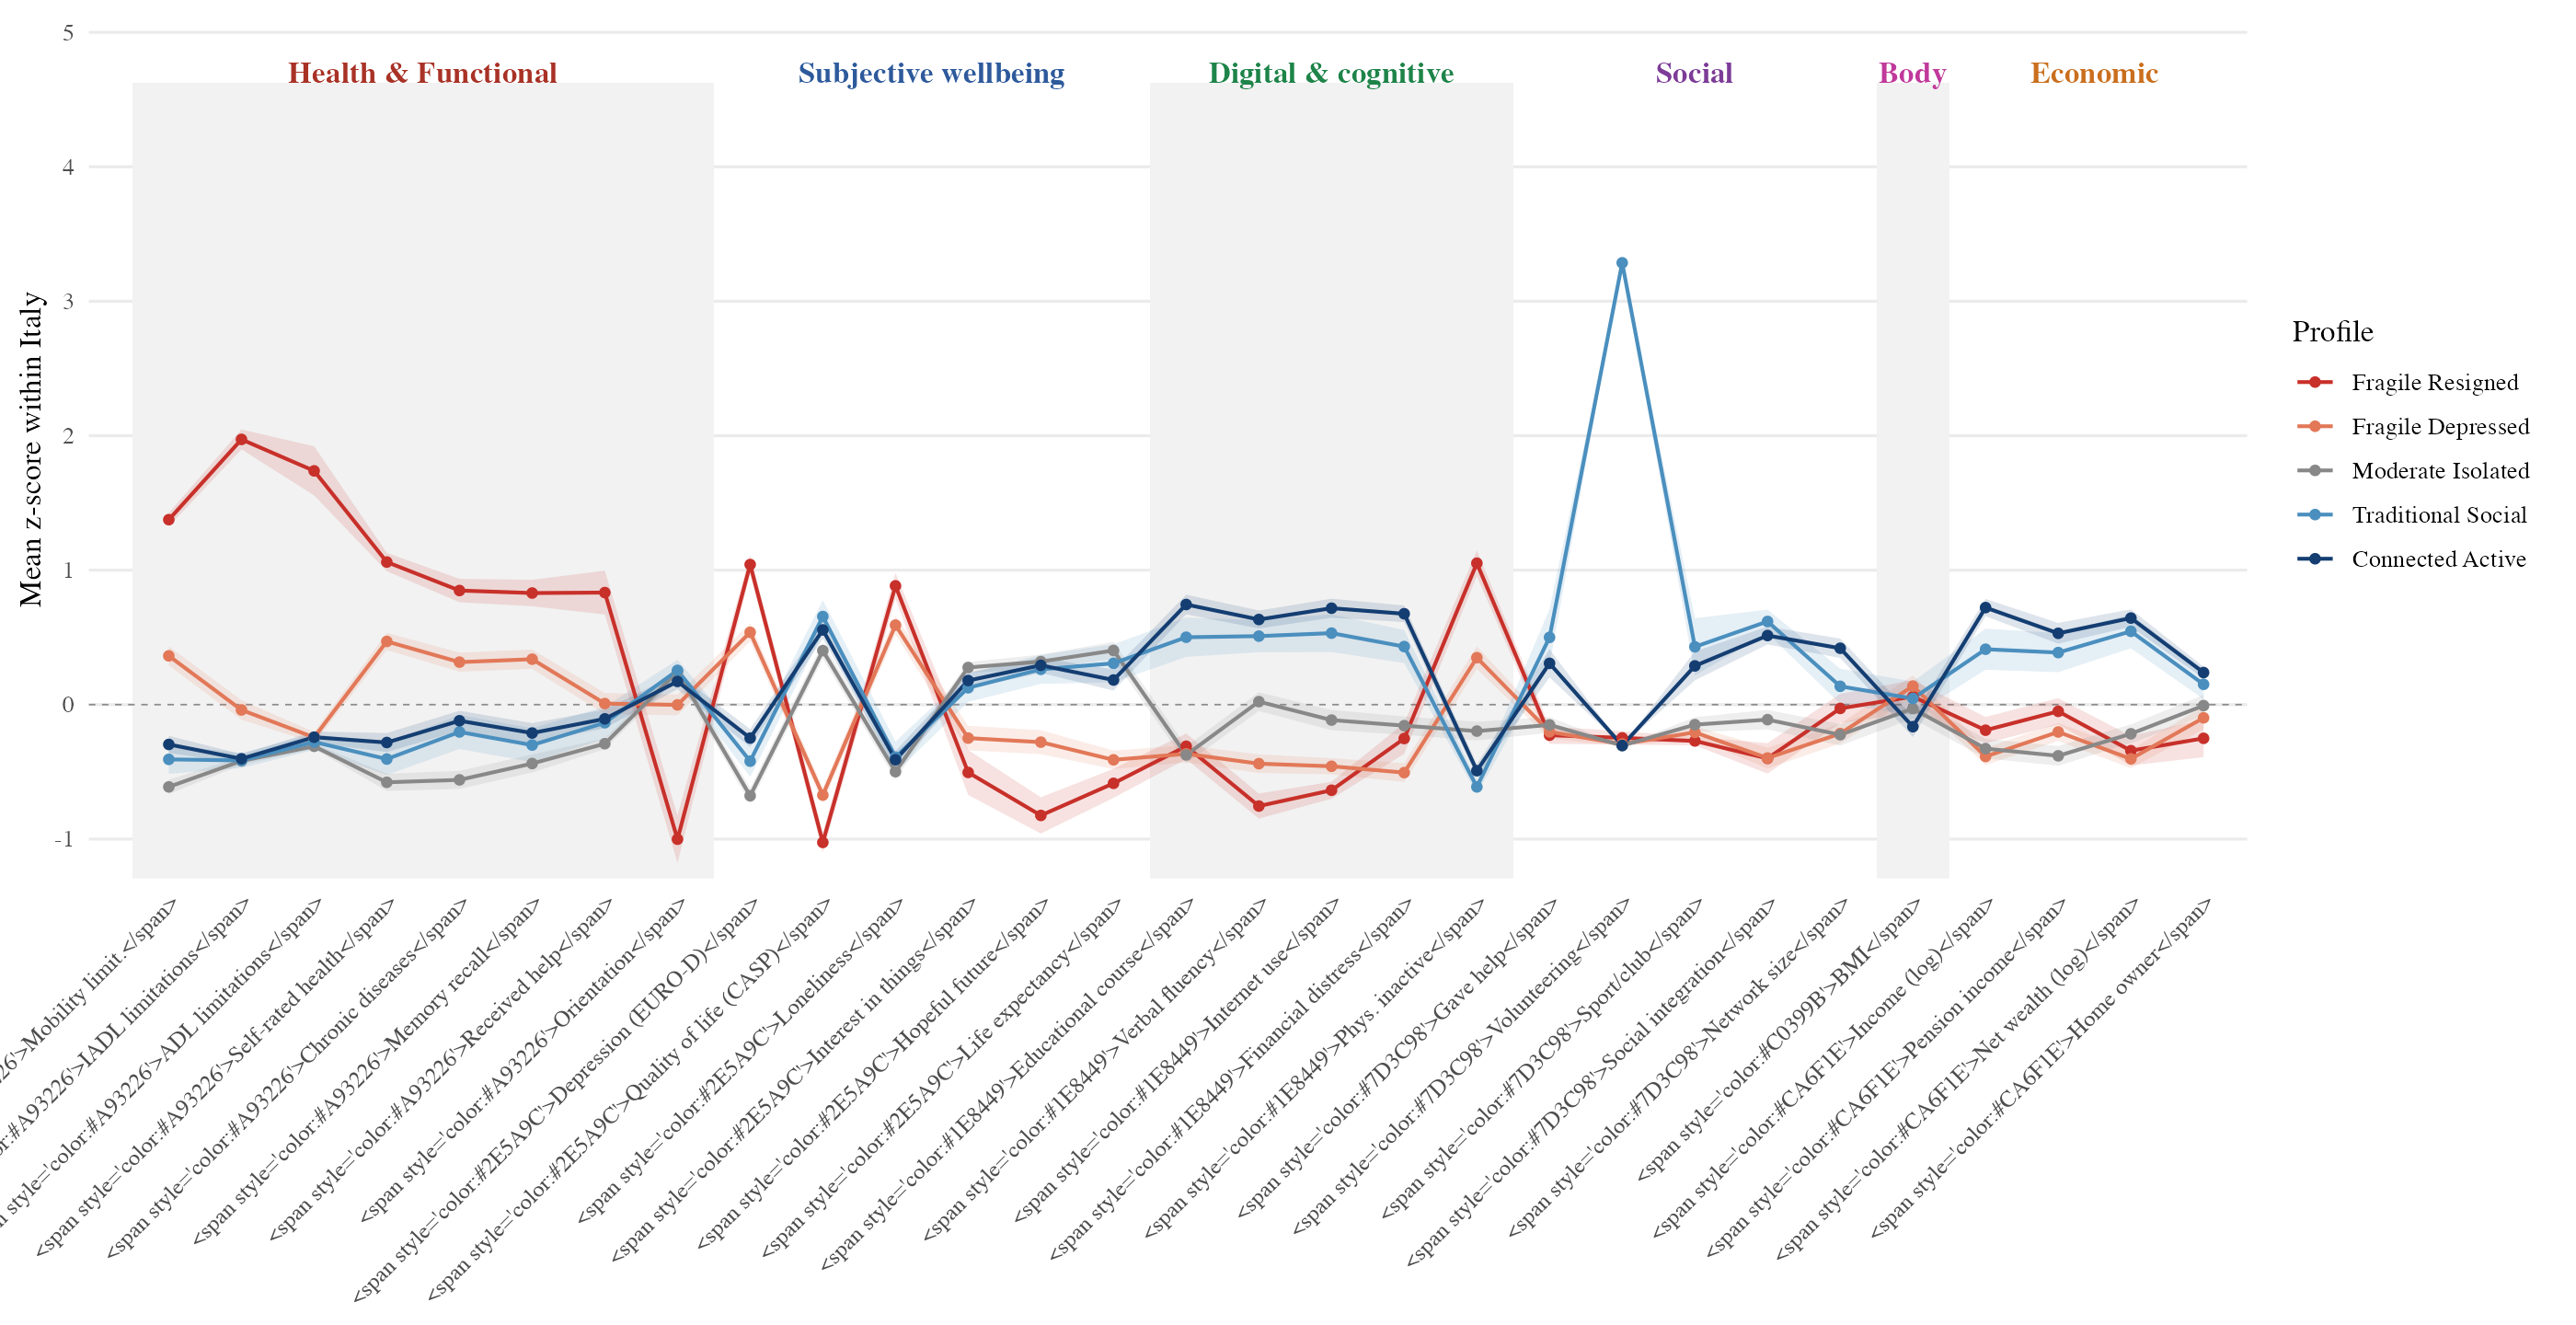
\includegraphics[width=0.95\linewidth]{figures/04_italy/fig_fingerprint_facet_italy.png}
  \caption{Profile fingerprint, Italy. Mean z-score per profile across the 29 active analytical variables, with 95\% bootstrap confidence ribbons ($n = 2{,}378$). Variables grouped by dominant Factor Analysis loading and ordered within factor; x-axis labels colour-coded by dimension.}
  \label{fig:ch4-fingerprint}
\end{figure}

\begin{figure}[ht]
  \centering
  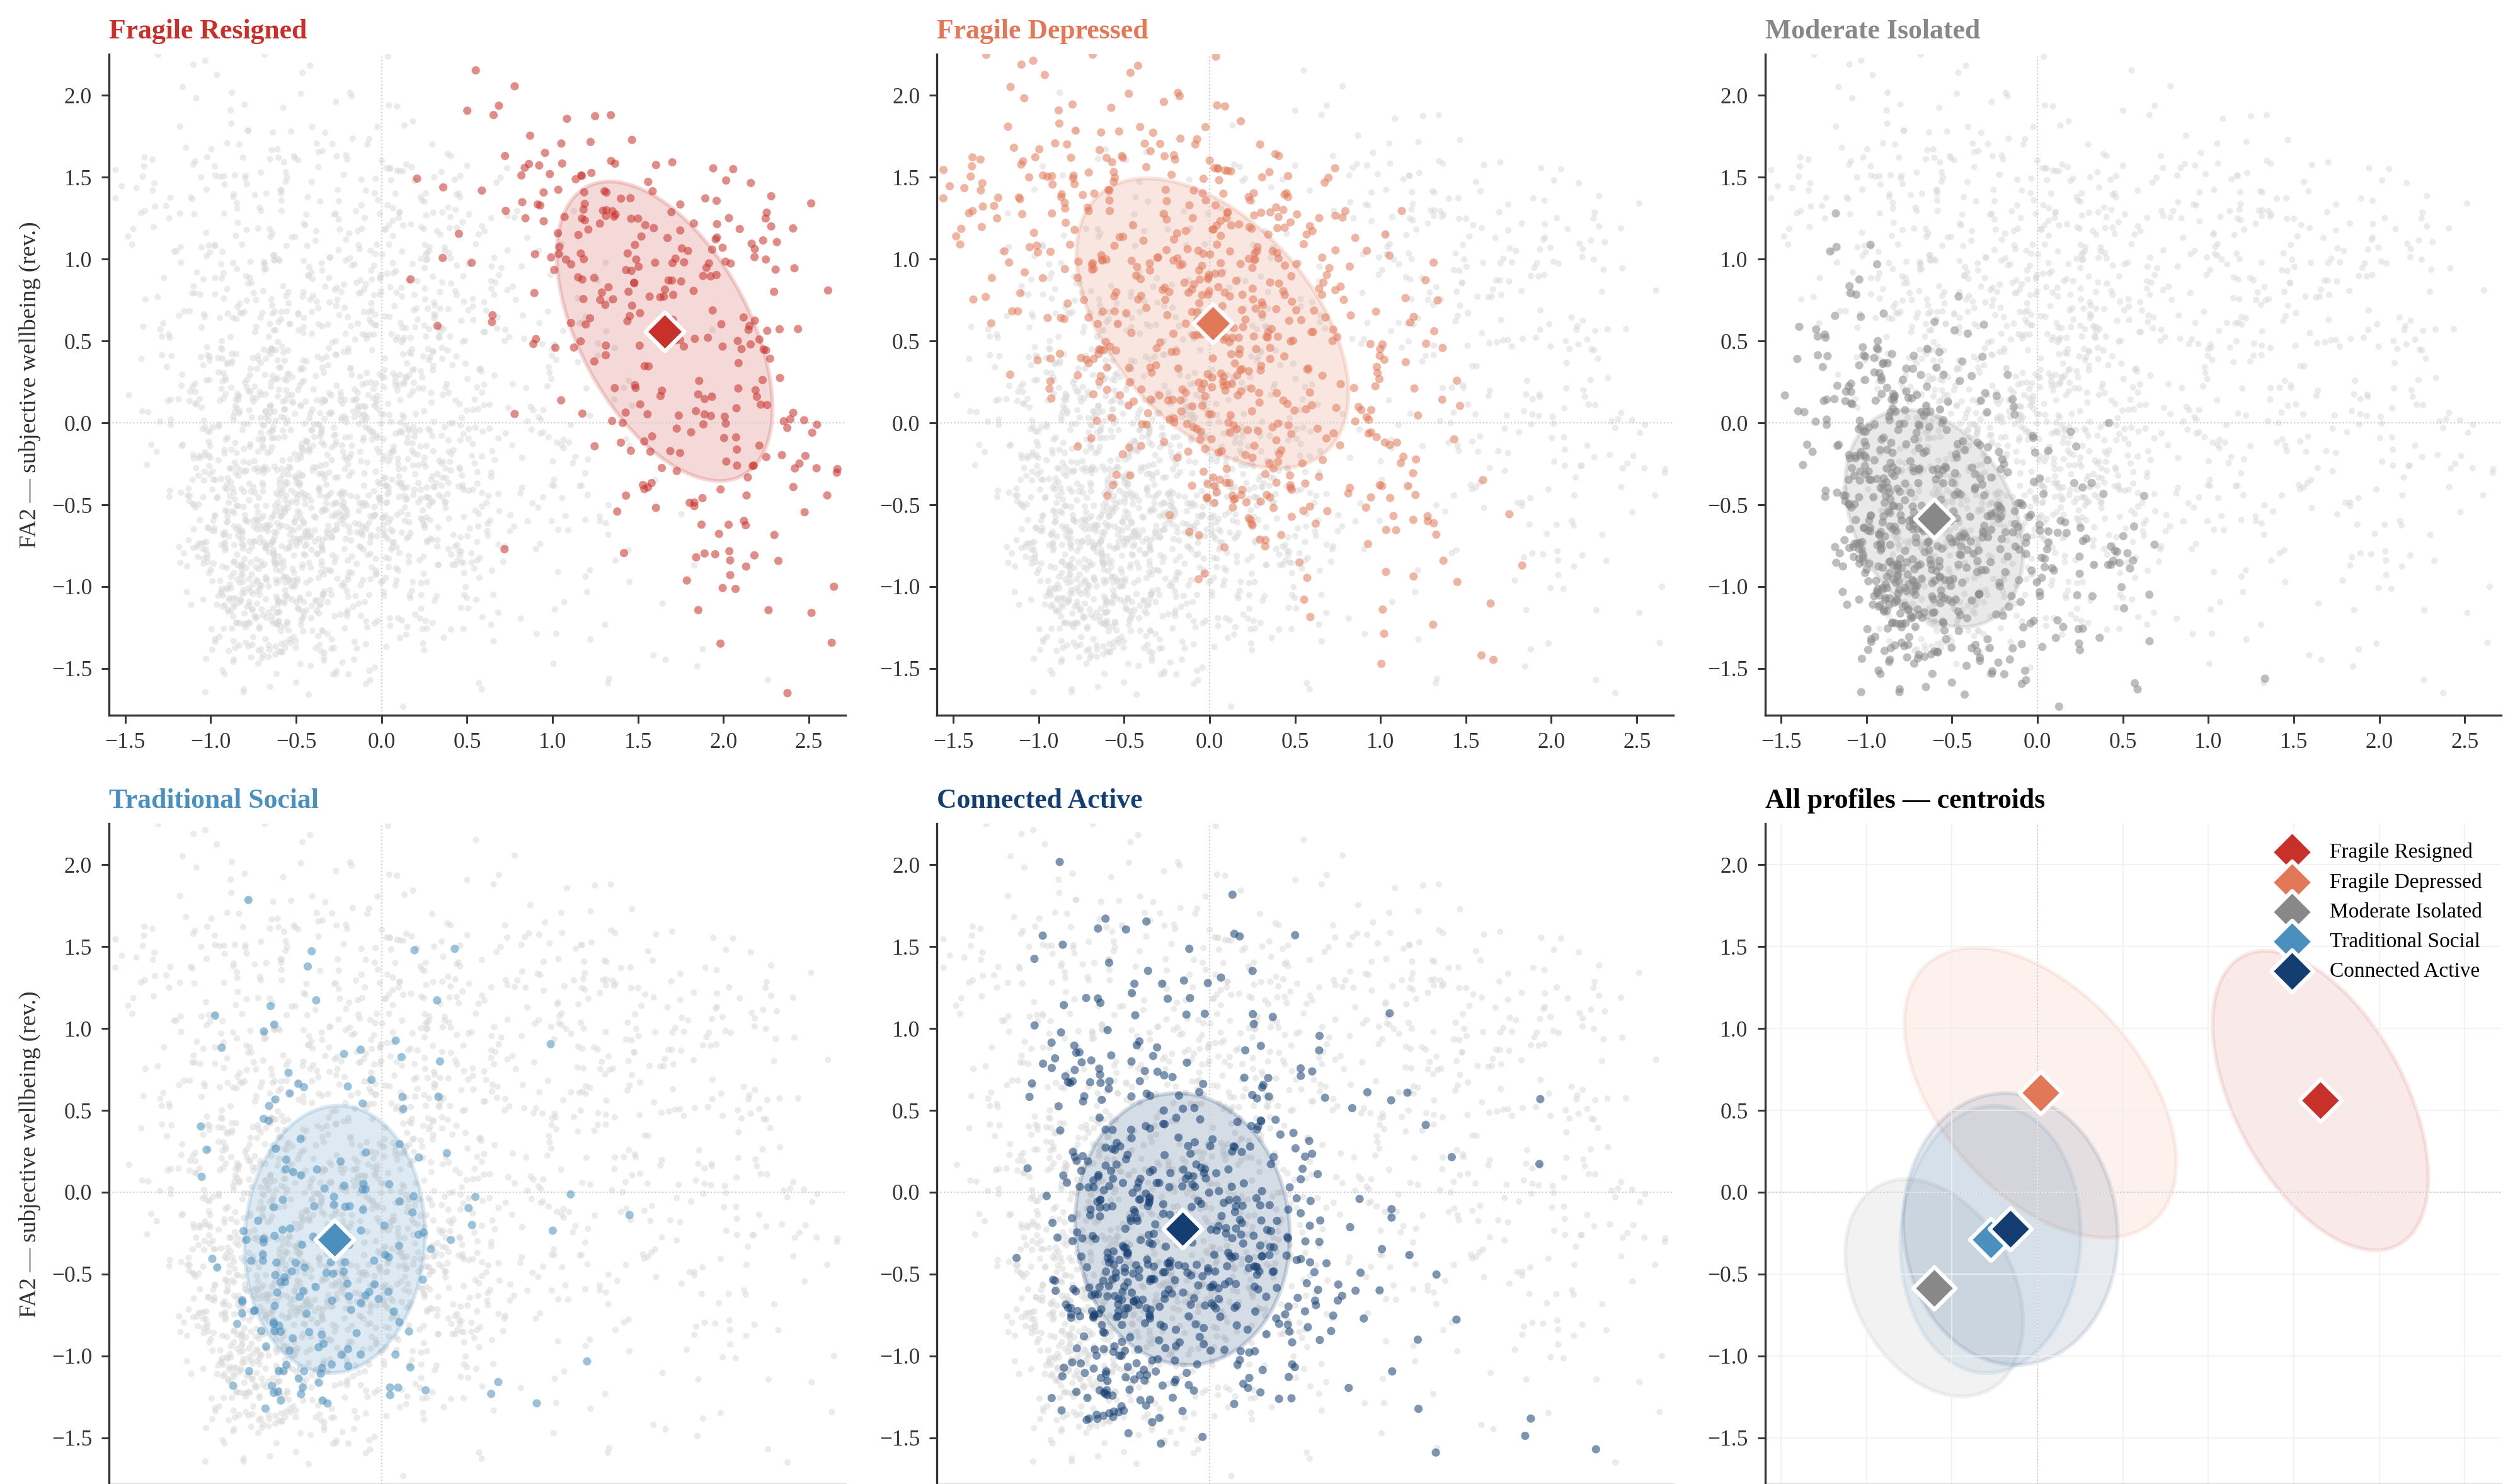
\includegraphics[width=0.95\linewidth]{figures/04_italy/fig_fa_scatter_pa1_pa2_italy.png}
  \caption{Profile scatter on the FA1 $\times$ FA2 plane, Italy. Each point is one Italian respondent positioned on the two dominant factors (FA1 = physical and functional fragility; FA2 = high values correspond to worse subjective wellbeing). Diamonds mark cluster centroids; ellipses mark 50\% confidence regions per profile.}
  \label{fig:ch4-fa-scatter}
\end{figure}

The visual reading of Figures~\ref{fig:ch4-fingerprint} and \ref{fig:ch4-fa-scatter} confirms the three-fold structure of the typology. The two fragile profiles lie above zero on health-burden variables and below zero on resource and digital variables, with Fragile Resigned systematically further from zero than Fragile Depressed. The Moderate Isolated and Traditional Social profiles overlap closely on resources and health and diverge sharply on social and digital engagement --- the country-specific Italian middle-stratum split. The Connected Active profile reaches the resource-and-digital pole on FA1 while remaining centred on FA2 --- the ``successful aging'' shape. The FA1 $\times$ FA2 scatter confirms that the five profiles occupy distinct regions of the latent space rather than a single severity gradient --- the visual counterpart of the substantive argument of \S\ref{sec:ch4-profile-descriptions}.

\section{External validation: life satisfaction}
\label{sec:ch4-external-validation}

Life satisfaction (SHARE Wave 9 item AC012, eleven-point scale) is administered in a separate questionnaire block and is not part of the analytical input set, providing an external validation outcome (Chapter~3). Figure~\ref{fig:ch4-lifesat} reports the distribution across the five Italian archetypes with the F-statistic of a one-way ANOVA in the figure caption.

\begin{figure}[ht]
  \centering
  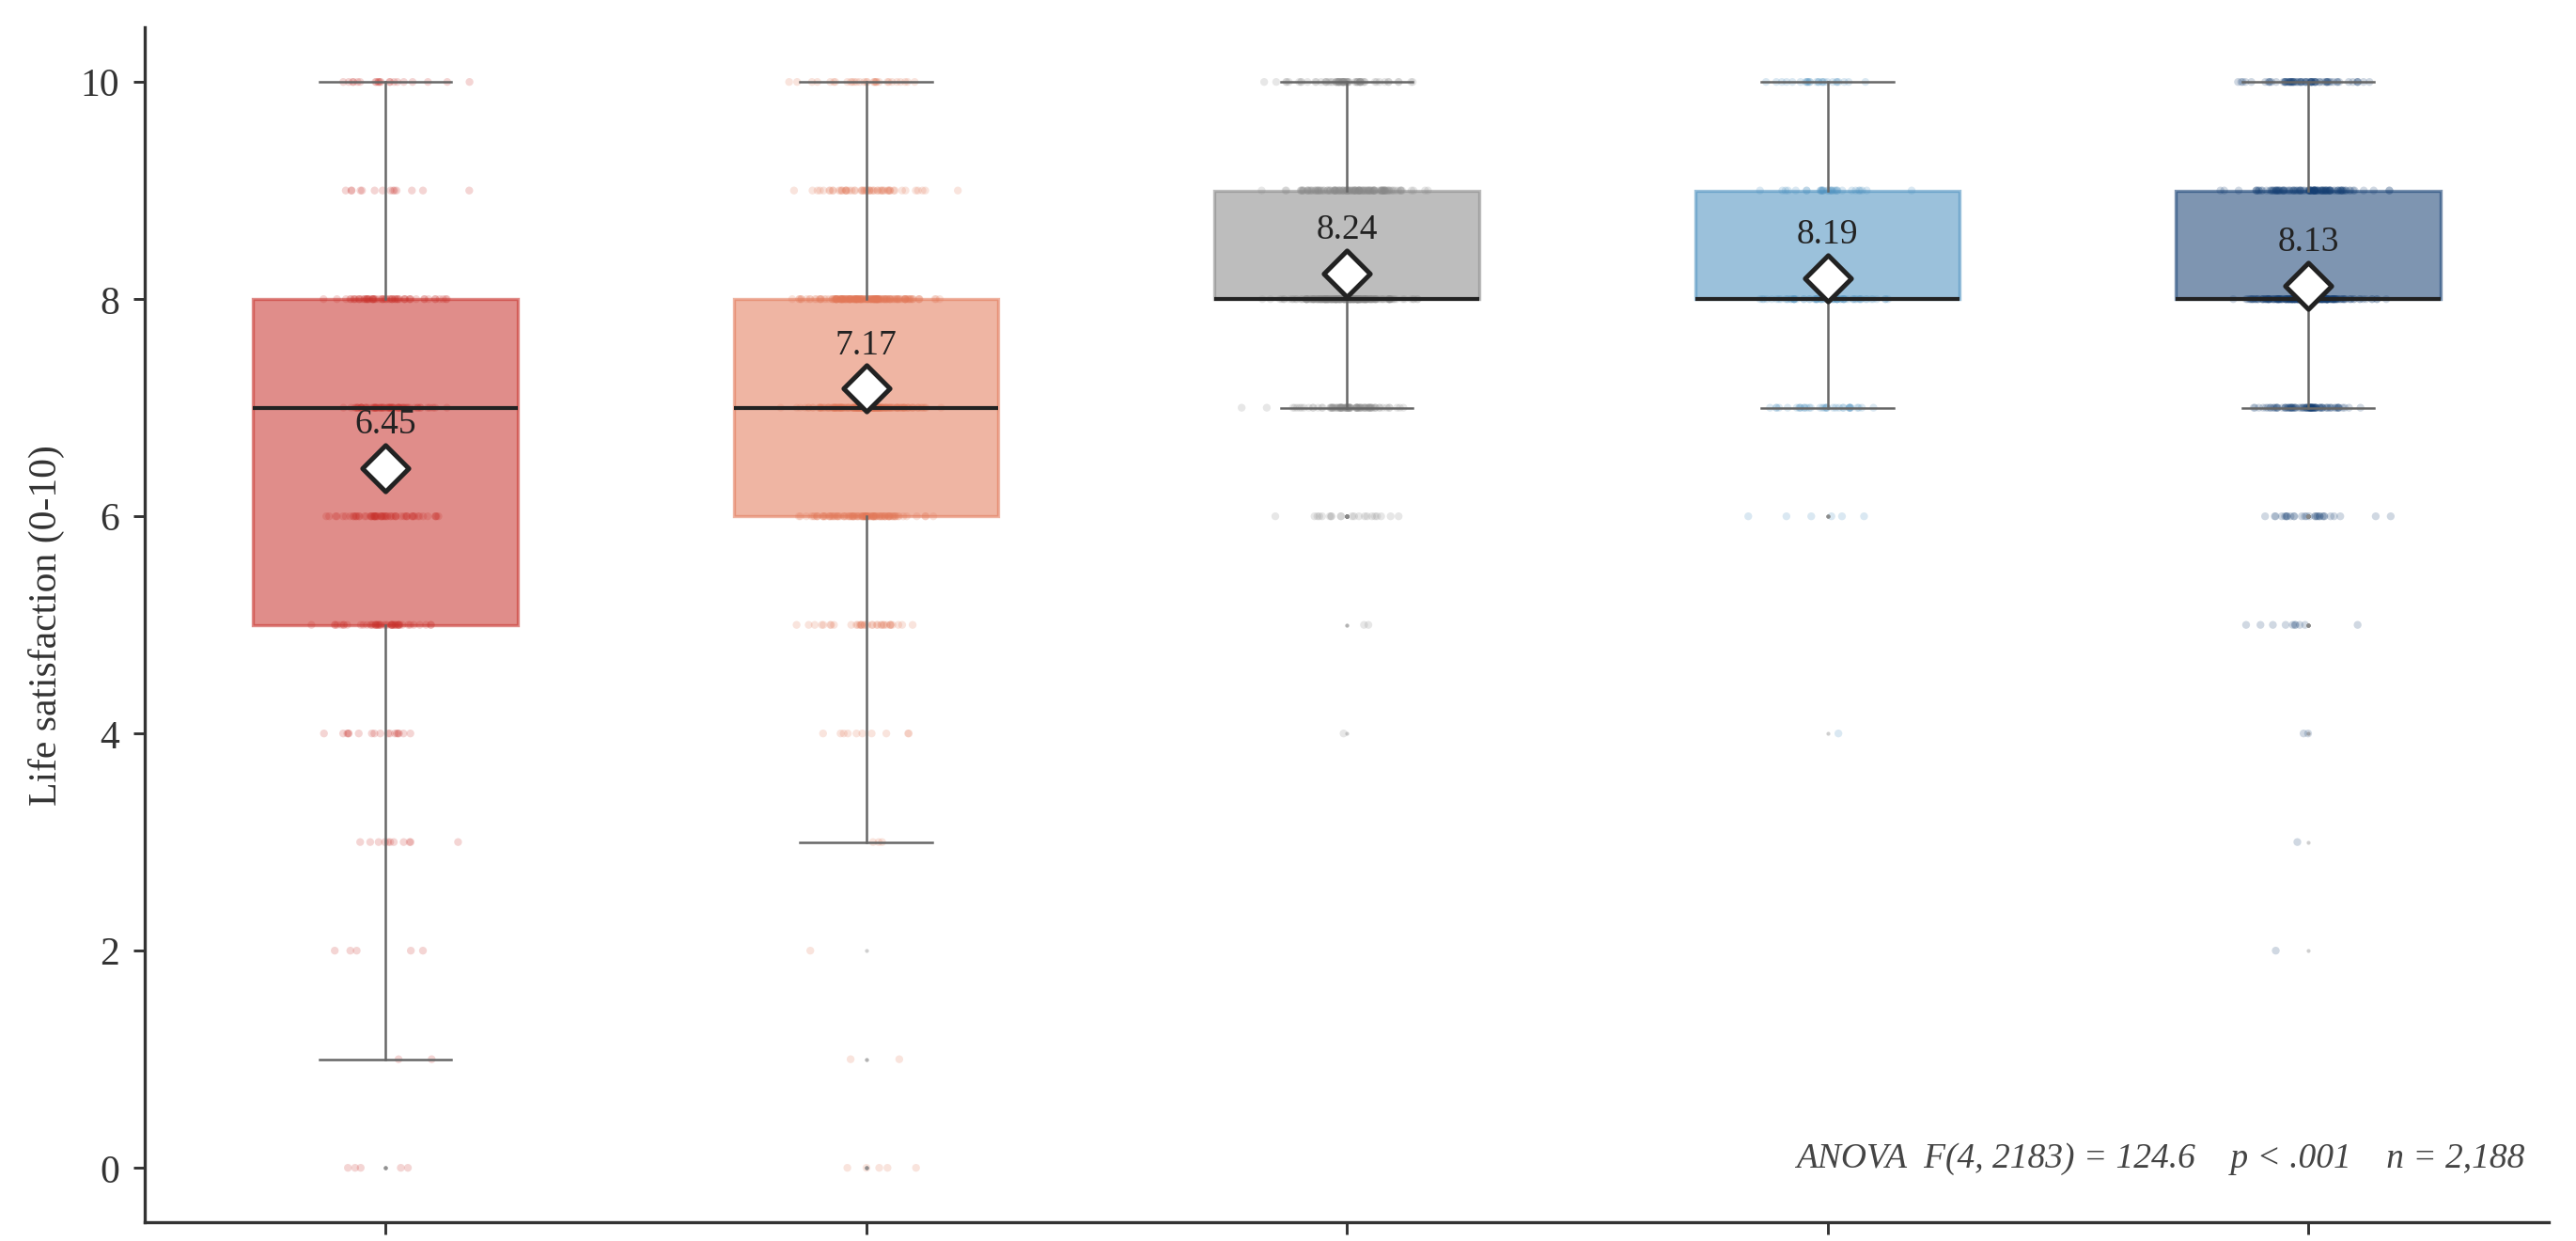
\includegraphics[width=0.95\linewidth]{figures/04_italy/fig_lifesat_anova_italy.png}
  \caption{Life satisfaction by profile, Italy. Boxplots of SHARE Wave 9 item AC012 (eleven-point scale, 0--10) by cluster membership; diamonds report cluster means. One-way ANOVA: $F(4, 2183) = 124.6$, $p < .001$. $n = 2{,}188$ (item-level non-response on lifesat reduces the analytical sample by 190 respondents from the 2,378 used for the segmentation).}
  \label{fig:ch4-lifesat}
\end{figure}

Mean life satisfaction is 6.5 in Fragile Resigned, 7.2 in Fragile Depressed, and clusters around 8.1--8.2 in the three non-fragile profiles, which are not statistically distinguishable from each other on this single item. The F-statistic of 124.6 on (4, 2183) degrees of freedom ($p < 0.001$) confirms substantial discriminative power of the typology on an outcome external to the input set. The lifesat outcome detects principally the binary contrast between fragile and non-fragile profiles (a roughly 1.5-point gap on the eleven-point scale); the within-non-fragile contrasts are minor --- consistent with the observation that life satisfaction in older age is dominated by the absence of major health and affective burdens. This supports the inclusion of the affective and evaluative subjective block as a constituent input to the typology, which preserves the within-fragile contrast (Fragile Resigned vs Fragile Depressed) that the lifesat outcome alone would not.

\section{Demographic distributions across profiles}
\label{sec:ch4-demographics}

The five archetypes are not uniformly distributed across gender and age. Figure~\ref{fig:ch4-gender} reports profile composition by gender on a 100\% stacked bar; Figure~\ref{fig:ch4-age} reports the parallel decomposition by age band (65--74, 75--84, 85+).

\begin{figure}[ht]
  \centering
  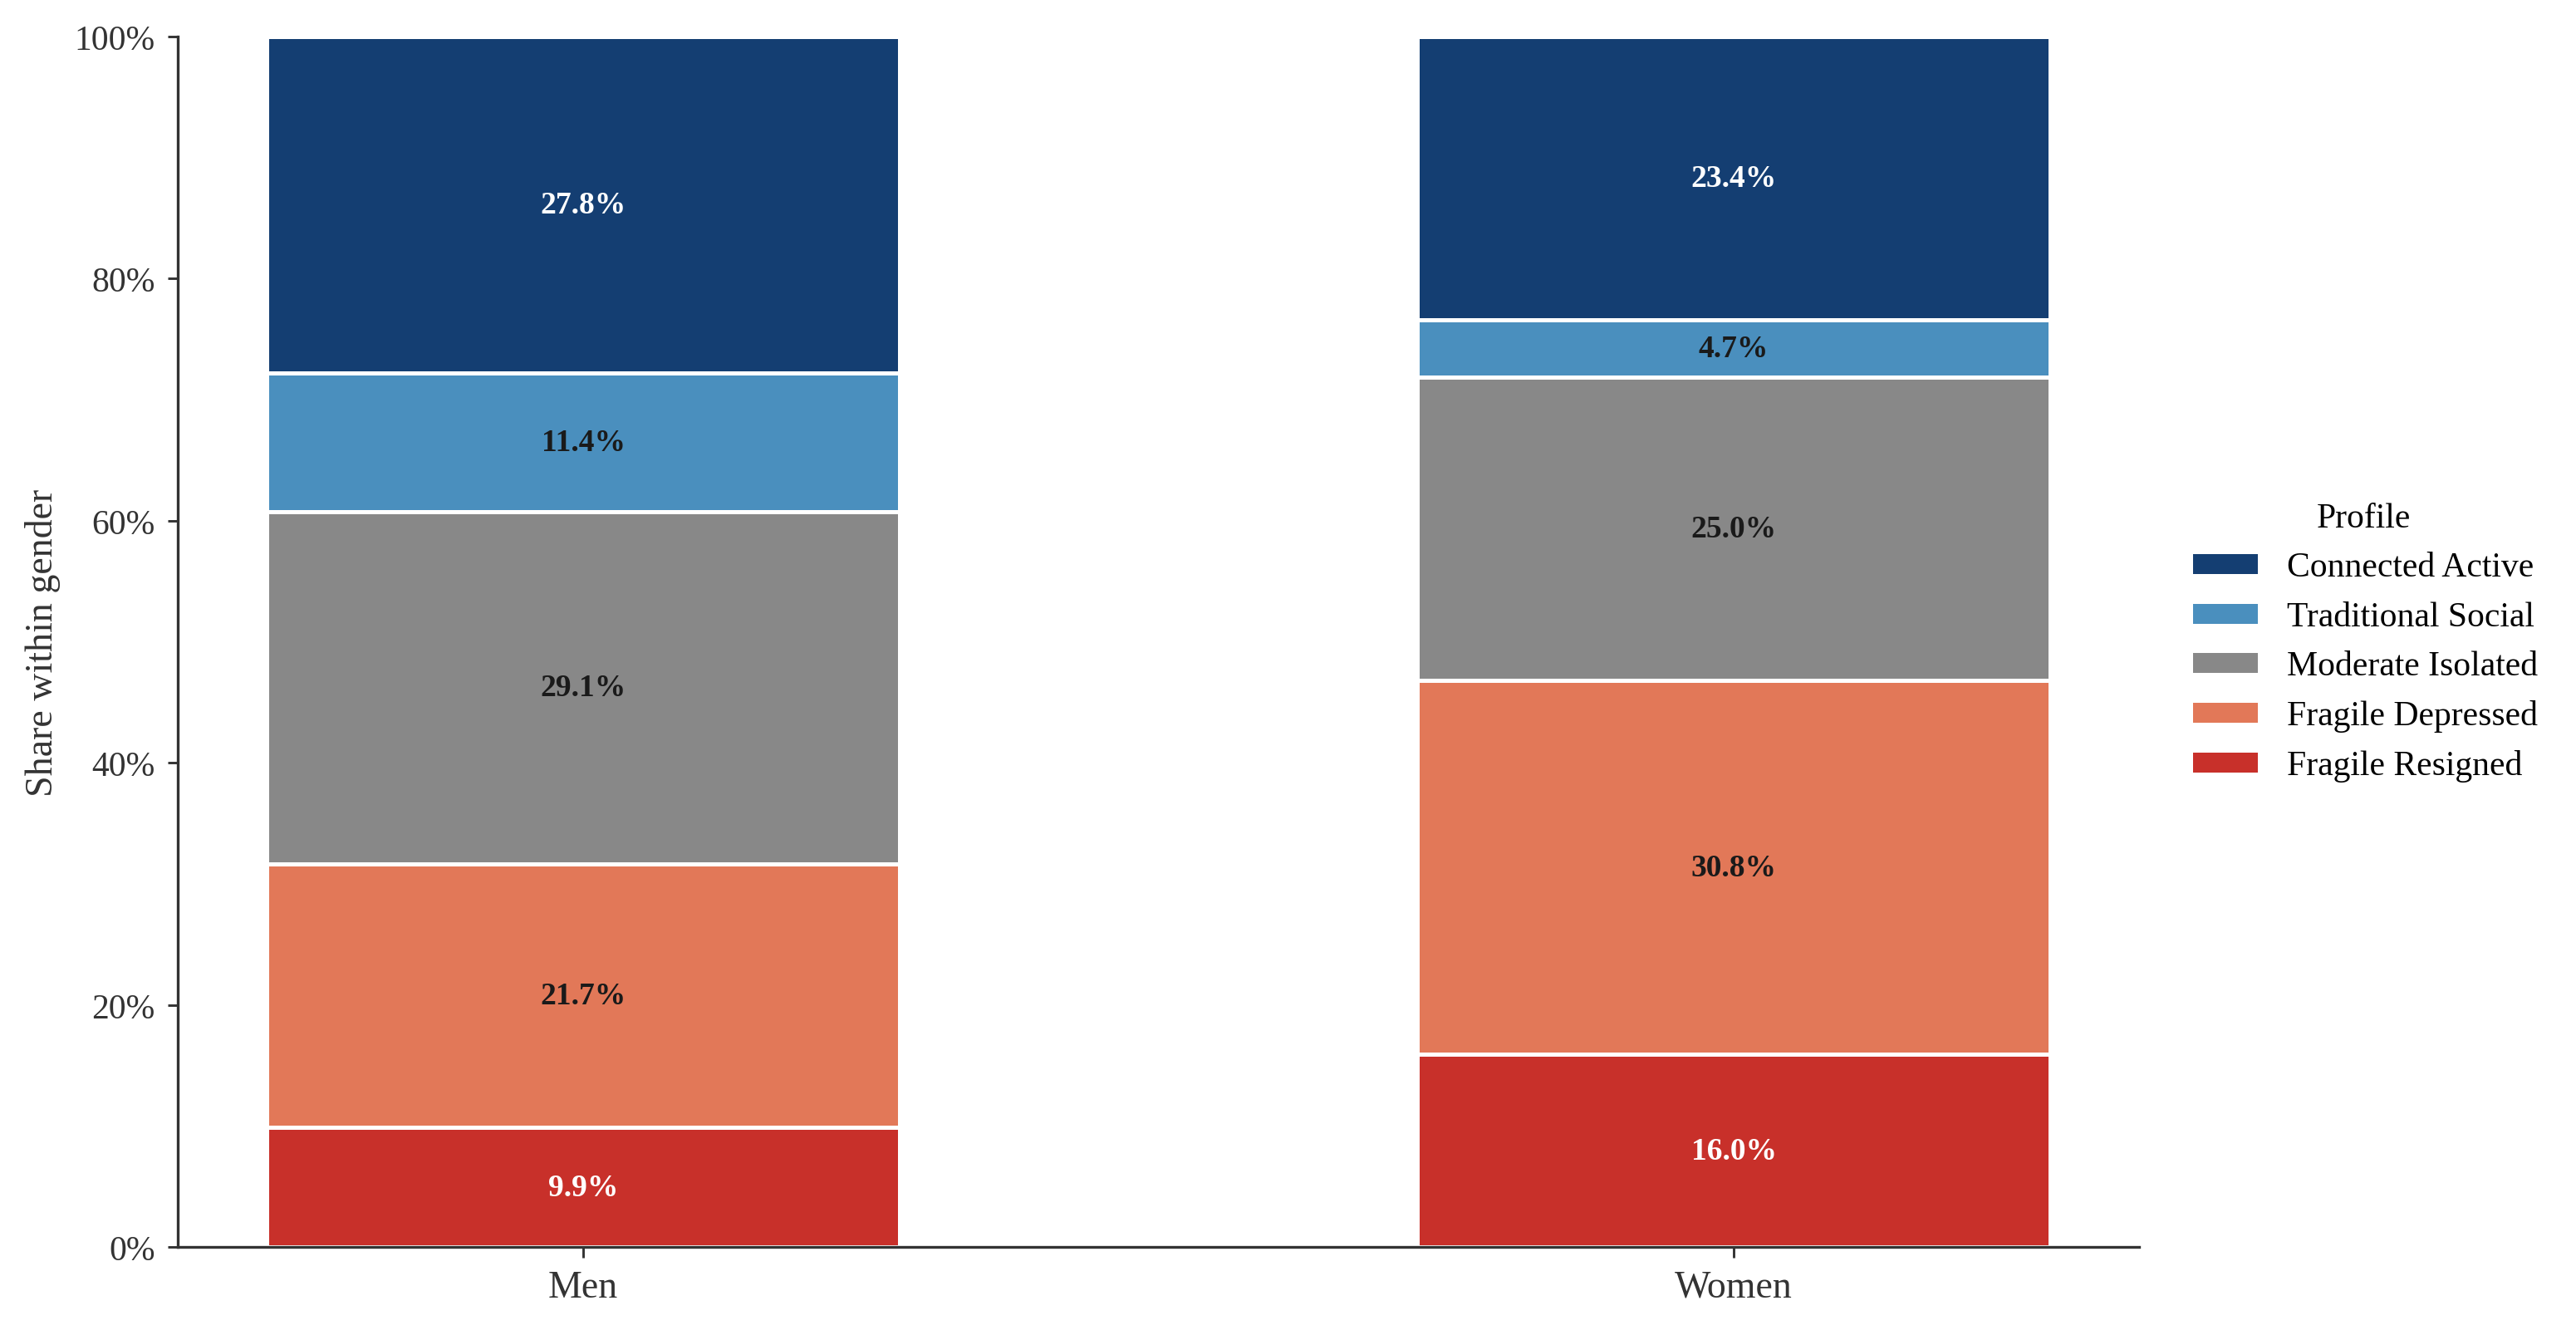
\includegraphics[width=0.95\linewidth]{figures/04_italy/fig_demographics_gender_italy.png}
  \caption{Profile composition by gender, Italy. Each column shows the percentage of the gender group falling in each archetype; columns sum to 100\%.}
  \label{fig:ch4-gender}
\end{figure}

\begin{figure}[ht]
  \centering
  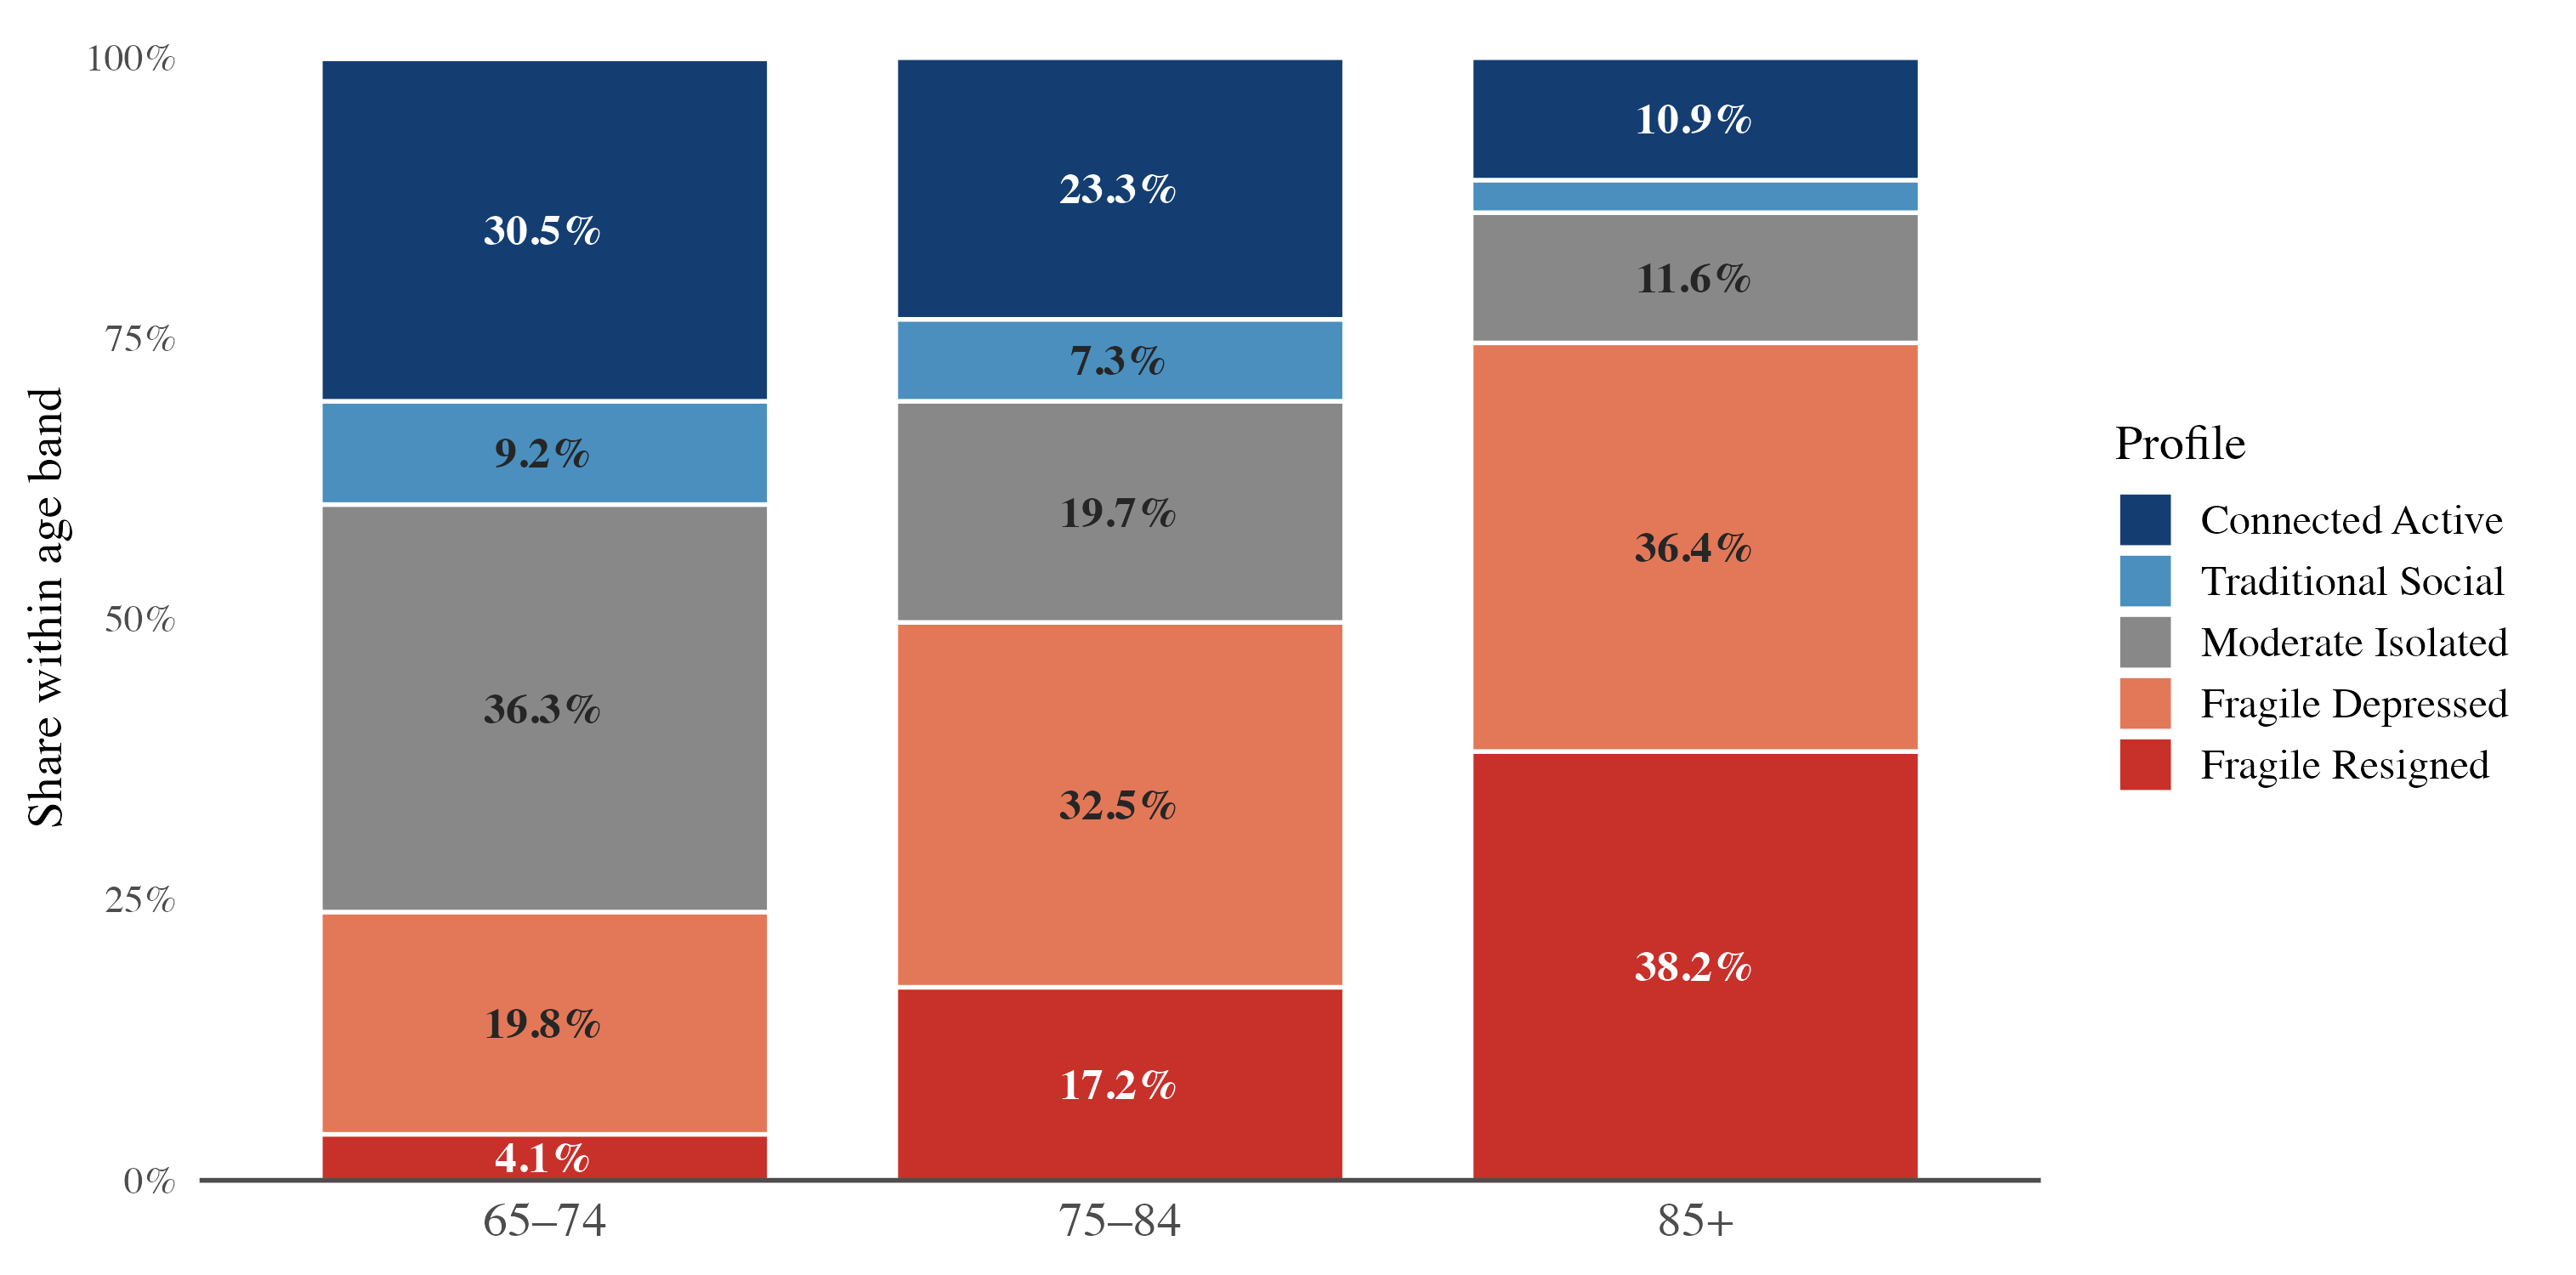
\includegraphics[width=0.95\linewidth]{figures/04_italy/fig_demographics_age_italy.png}
  \caption{Profile composition by age band, Italy. The Fragile Resigned share rises from 4\% in 65--74 to 38\% in 85+; the Connected Active share declines from 31\% to 11\% over the same range.}
  \label{fig:ch4-age}
\end{figure}

Two patterns emerge. First, the feminisation of fragility: 47\% of Italian over-65 women fall in one of the two fragile profiles (16\% Fragile Resigned + 31\% Fragile Depressed), against 32\% of men (10\% + 22\%). Conversely, 39\% of men are in the high-resource profiles (28\% Connected Active + 11\% Traditional Social), against 28\% of women. The pattern is consistent with the broader epidemiological literature on the differential aging of Italian women --- longer life expectancy paired with higher widowhood rates, lower lifetime labour-market attachment, lower individual pension income \citep{dykstra2009, pampel2001}.

Second, the age gradient is strong. In the 65--74 band, 31\% of respondents are in the Connected Active cluster and only 4\% in Fragile Resigned; in the 85+ band, the proportions are reversed (11\% Connected Active, 38\% Fragile Resigned). The Fragile Depressed share also increases monotonically with age (20\% $\to$ 33\% $\to$ 36\%); the Moderate Isolated share declines from 36\% to 12\%, reflecting the cohort transition from socially-disengaged but functionally autonomous late-young-old to functionally impaired oldest-old respondents. The most vulnerable sub-population (women, oldest old, fragile) is also the sub-population for whom standard digital channels of the silver economy are essentially inaccessible without family or institutional intermediation --- a finding with direct implications for the design of long-term-care services and digital products targeting the Italian over-65 population.

\section{The Isolation Paradox}
\label{sec:ch4-isolation-paradox}

The most distinctive finding of the Italian typology --- and one of the three original contributions of this thesis articulated in Chapter~1 --- is what we term the Isolation Paradox: the existence in Italy of a substantial population segment that is functionally and economically autonomous but socially and digitally disconnected, and that systematically under-utilises the healthcare system relative to peers with comparable health and resources but denser social engagement. The segment is the Moderate Isolated archetype described in \S\ref{sec:ch4-moderate-isolated}, with 28.1\% population share and approximately 3.98 million individuals.

\subsection{The empirical signature}
\label{sec:ch4-isolation-empirical}

The Moderate Isolated cluster shares with the Traditional Social cluster three core configurations: comparable health (mobility 0.6 vs 0.9 raw count, EURO-D 1.2 vs 1.7), comparable economic resources (log\_thinc within 0.7 z-score units), and comparable subjective evaluation of life (CASP 36.8 vs 38.5; both above the Italian mean). The two clusters diverge sharply on the social, cultural and digital engagement dimensions: the Moderate Isolated cluster is at $z = -0.22$ on network size against $+0.14$ for Traditional Social; at $z = -0.11$ on internet use against $+0.53$ for Traditional Social; at $z$ between $-0.15$ and $-0.37$ on cultural-engagement indicators against $+0.43$ to $+3.29$. In raw figures: 2.3 confidants vs 2.6, 34.1\% internet use vs 65.8\%, half the cultural-event participation rate. Despite these differences, the two clusters report the same mean life satisfaction (8.2 vs 8.2) --- the social isolation is not internalised as a deficit by the affected individuals on standard subjective-well-being indicators.

\subsection{The healthcare under-utilisation pattern}
\label{sec:ch4-isolation-healthcare}

The Isolation Paradox is substantiated by the analysis of healthcare utilisation across the two middle-stratum clusters, reported in detail in Chapter~6. Relative to Traditional Social, Moderate Isolated reports 1.36 fewer doctor visits per year, 0.72 fewer specialist visits, a 0.4 percentage-point higher rate of forgone care (respondents who report having needed but not received medical attention), and 2.02 fewer nights in hospital per year. The pattern is consistent across age bands and regions and survives adjustment for chronic-condition count, self-rated health, and economic resources. The combined effect is a systematic disengagement from the formal healthcare system, with the segment dropping below population averages on preventive, outpatient and inpatient indicators alike --- a configuration consistent with structural detachment from care channels rather than with delayed care-seeking.

\begin{figure}[ht]
  \centering
  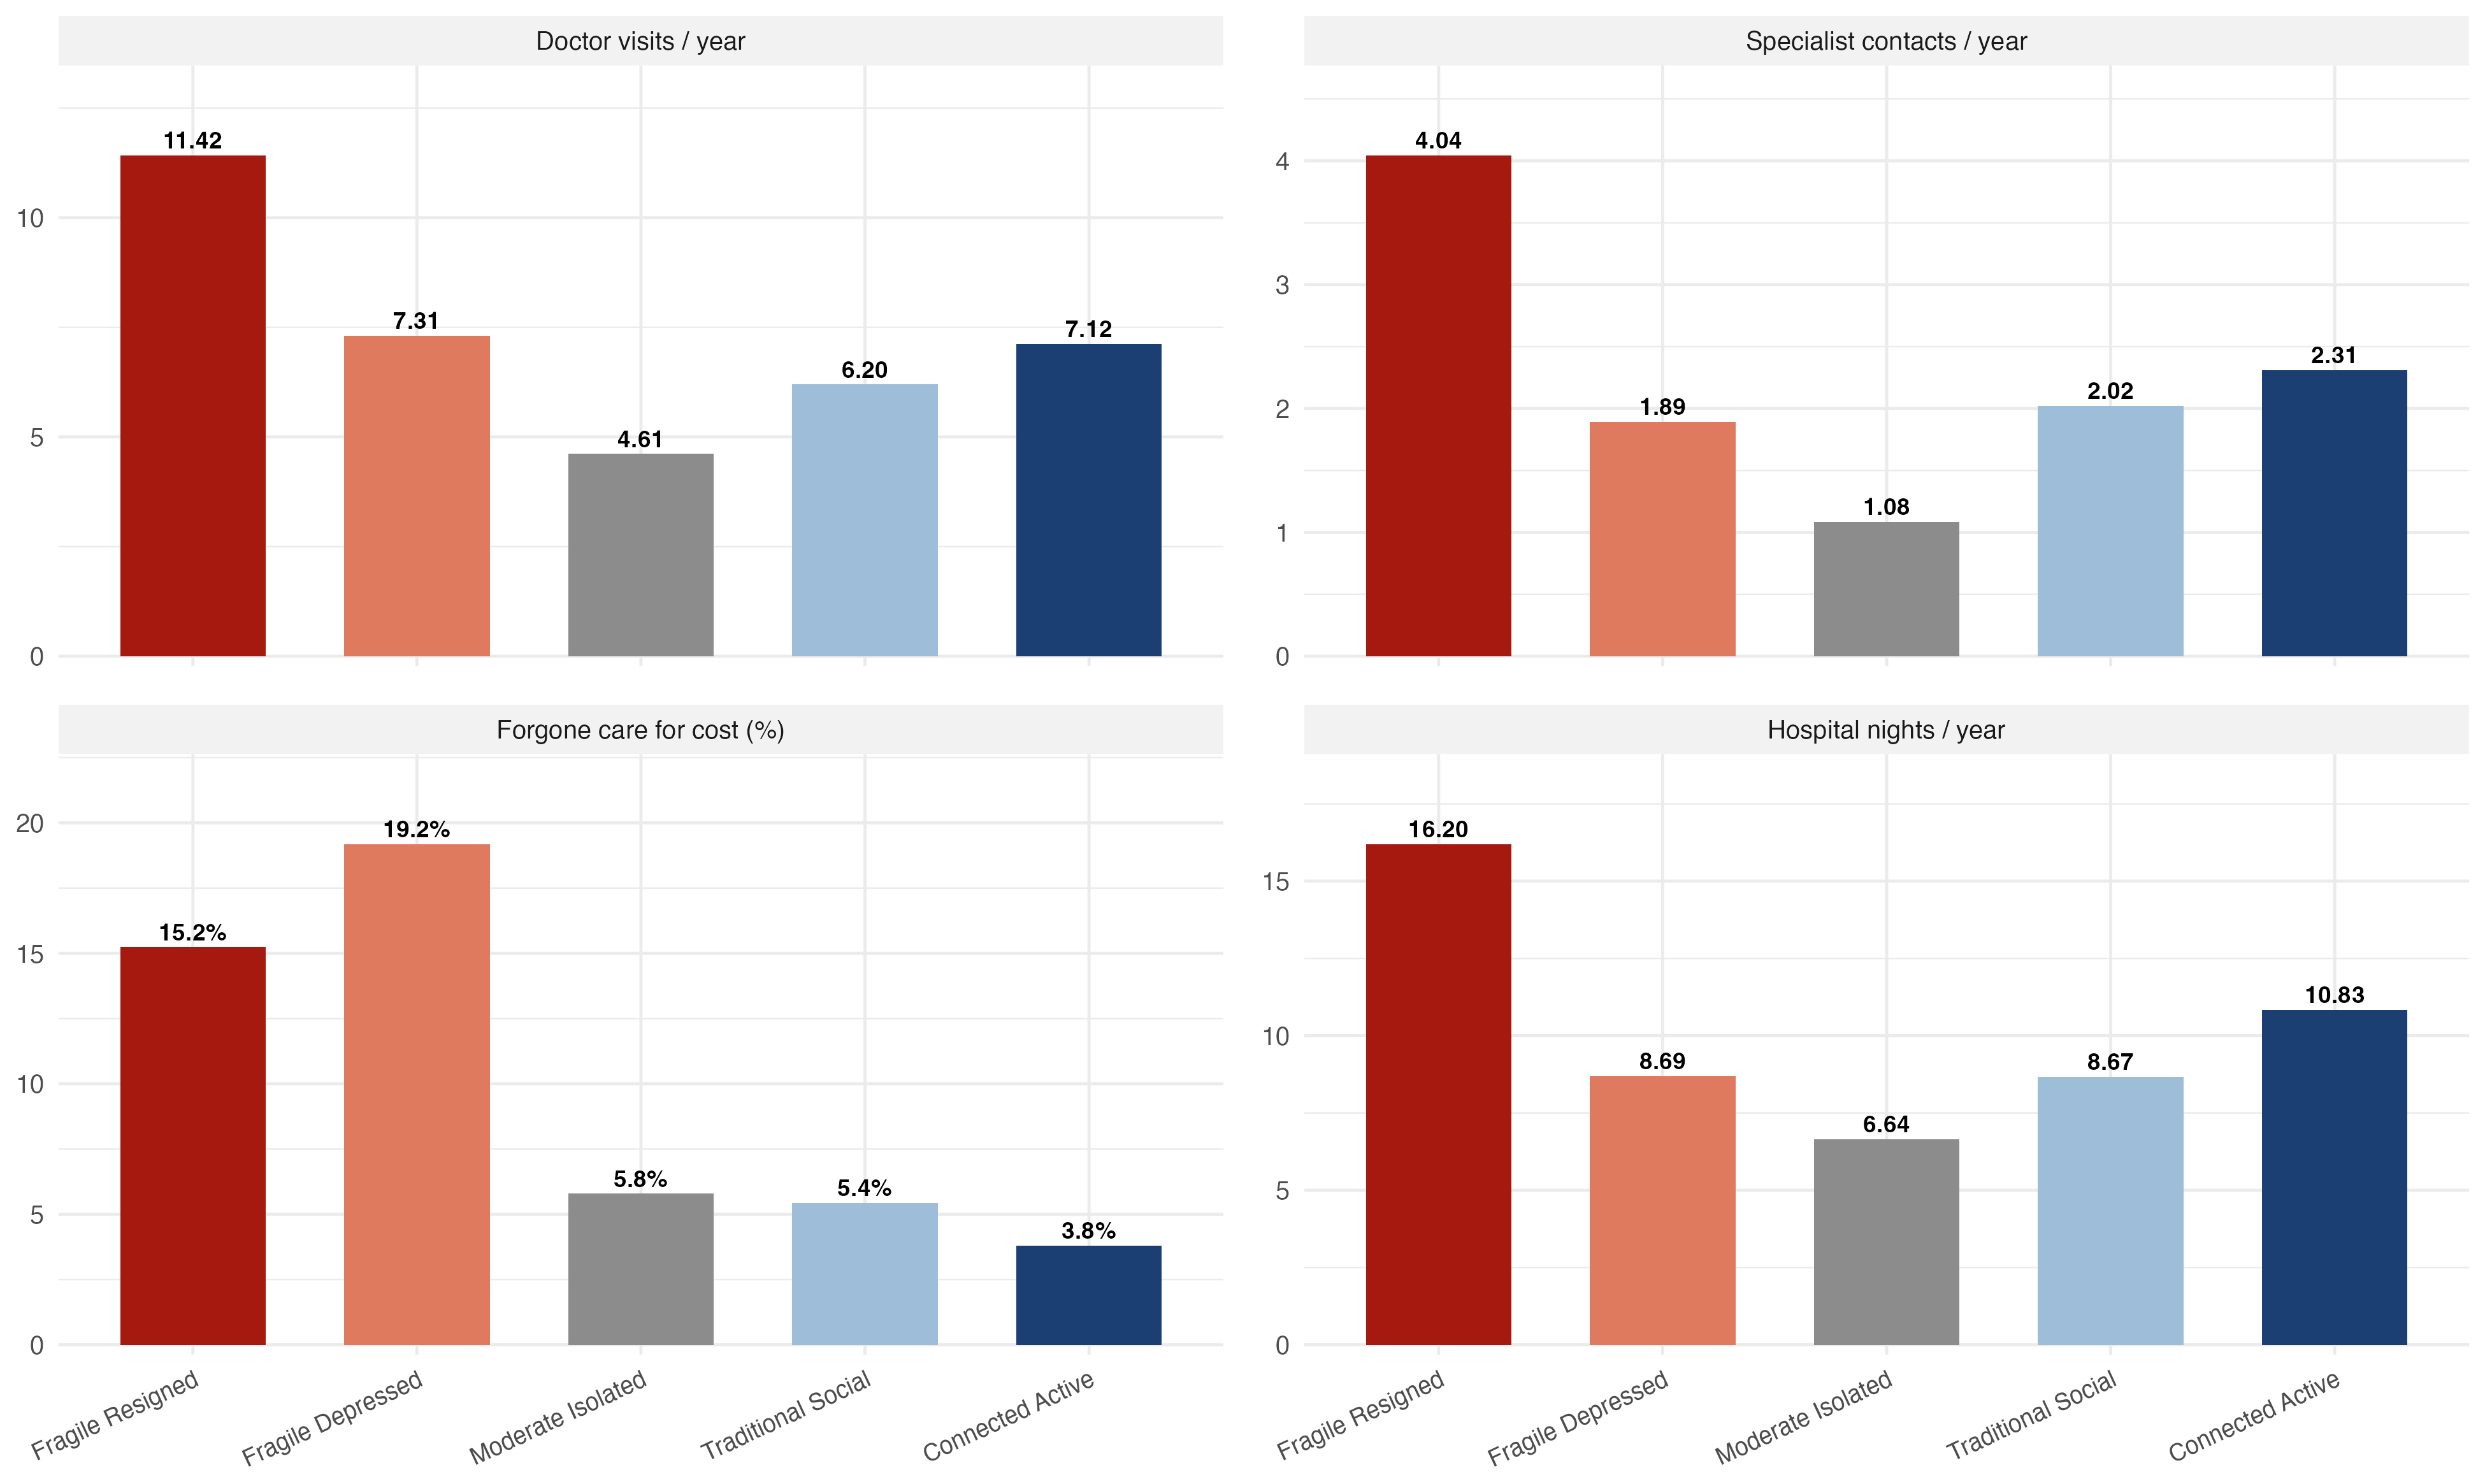
\includegraphics[width=0.95\linewidth]{figures/04_italy/fig_healthcare_italy.png}
  \caption{Healthcare utilisation across the five Italian archetypes. Cluster means on four healthcare indicators (doctor visits, specialist visits, forgone care percentage, hospital nights). Note the Moderate Isolated under-utilisation of preventive and outpatient care paired with over-utilisation of inpatient care --- the empirical signature of the Isolation Paradox (\S\ref{sec:ch4-isolation-paradox}).}
  \label{fig:ch4-healthcare}
\end{figure}

The mechanism is consistent with three convergent literatures. The literature on social capital and healthcare access \citep{berkmankawachi2000, putnam2000} documents the role of dense social networks in transmitting symptom information and signposting individuals towards appropriate care. The gerontological literature on the gateway role of grandchildren and adult children in mediating digital and informational access of older adults \citep{quanhaase2017} identifies a role that the Moderate Isolated cluster, with its thin family-network structure, is by definition unable to leverage. The Italian welfare-state literature on regional fragmentation of public health services \citep{loscalzo2009} makes informal social capital a more critical input for healthcare navigation than in welfare regimes designed for universal access.

\subsection{Why the Paradox is Italian-only}
\label{sec:ch4-isolation-italian-only}

The Isolation Paradox does not have a structural counterpart in the Swedish typology of Chapter~5. The Swedish Moderate archetype is socially integrated at a level comparable to the Swedish population mean, with internet use above 90\% and network size at the population mean. The Hungarian-matched cross-country analysis of Chapter~6 confirms that the Moderate Isolated cluster has no Swedish twin within a structural distance $\leq 2.0$ in standardised space --- it is a country-specific Italian phenomenon. The reading is that the Moderate Isolated configuration emerges where the welfare regime substitutes individual responsibility and family-based provision for universal-access institutions \citep{espingandersen1990, ferrera1996}. In Italy, individuals not embedded in a dense family or community network face a thin informational environment and a fragmented public-service infrastructure; in Sweden, the universal-access infrastructure provides a substitute baseline that prevents the emergence of an analogous configuration.

\subsection{Policy and silver-economy implications}
\label{sec:ch4-isolation-implications}

The Isolation Paradox has three implications for the design of services and technologies targeted at the Italian over-65 population. First, the size of the affected segment (3.98 million individuals) makes it a first-order policy and market reality, not a residual category. Second, the segment is not characterised by health or economic adversity that would route it into the existing long-term-care or income-support branches of the Italian welfare system; it is invisible to those branches. Third, the segment is not characterised by the absence of digital channels in absolute terms (34.1\% internet use is non-trivial); it is characterised by the absence of social and informational mediation that would route the available digital channels towards healthcare and service utilisation. The implication for silver-economy product design is that the Moderate Isolated segment is not addressable by direct-to-consumer digital products in the same way as the Connected Active segment; product designs that combine a digital channel with a social-mediation layer (peer-network platforms, community-based digital intermediaries, family-network-augmented service interfaces) are the candidate operational solution. The strategic case for this product-design gap as an opportunity for innovation in the Italian silver economy is developed in Chapter~6.

\section{Synthesis}
\label{sec:ch4-synthesis}

The Italian typology partitions the over-65 population into five archetypes spanning an interpretable severity gradient on health and resources, an orthogonal affective contrast within the fragile stratum, and an orthogonal cultural-versus-digital contrast within the high-resource stratum. The five archetypes are unequally distributed (28.1\% in the largest cluster, 11.7\% in the smallest), with population-projected sizes from 1.66 million (Fragile Depressed) to 3.98 million (Moderate Isolated). External validation against life satisfaction confirms substantial discriminative power ($F(4, 2183) = 124.6$, $p < 0.001$).

Three findings of substantive importance emerge. The qualitative distinction between Fragile Resigned and Fragile Depressed identifies two distinct configurations with different functional and affective signatures, calling for distinct policy responses (long-term-care provision in the first case, mental-health services in the second). The country-specific Moderate Isolated archetype --- the largest single cluster at 28.1\% --- identifies a substantial fraction of the Italian over-65 population whose late-life experience is socially and digitally thin. The Isolation Paradox documents that this segment, despite being functionally and economically autonomous, systematically under-utilises preventive and outpatient healthcare and over-utilises inpatient care, in a pattern consistent with the welfare-regime literature on Italian familism and the gerontological literature on social capital and healthcare access. The next chapter develops the parallel typology for Sweden; Chapter~6 maps the four matched cross-country pairs and develops the comparative reading of the Isolation Paradox; Chapter~7 reports the full battery of robustness diagnostics.

\begin{figure}[ht]
  \centering
  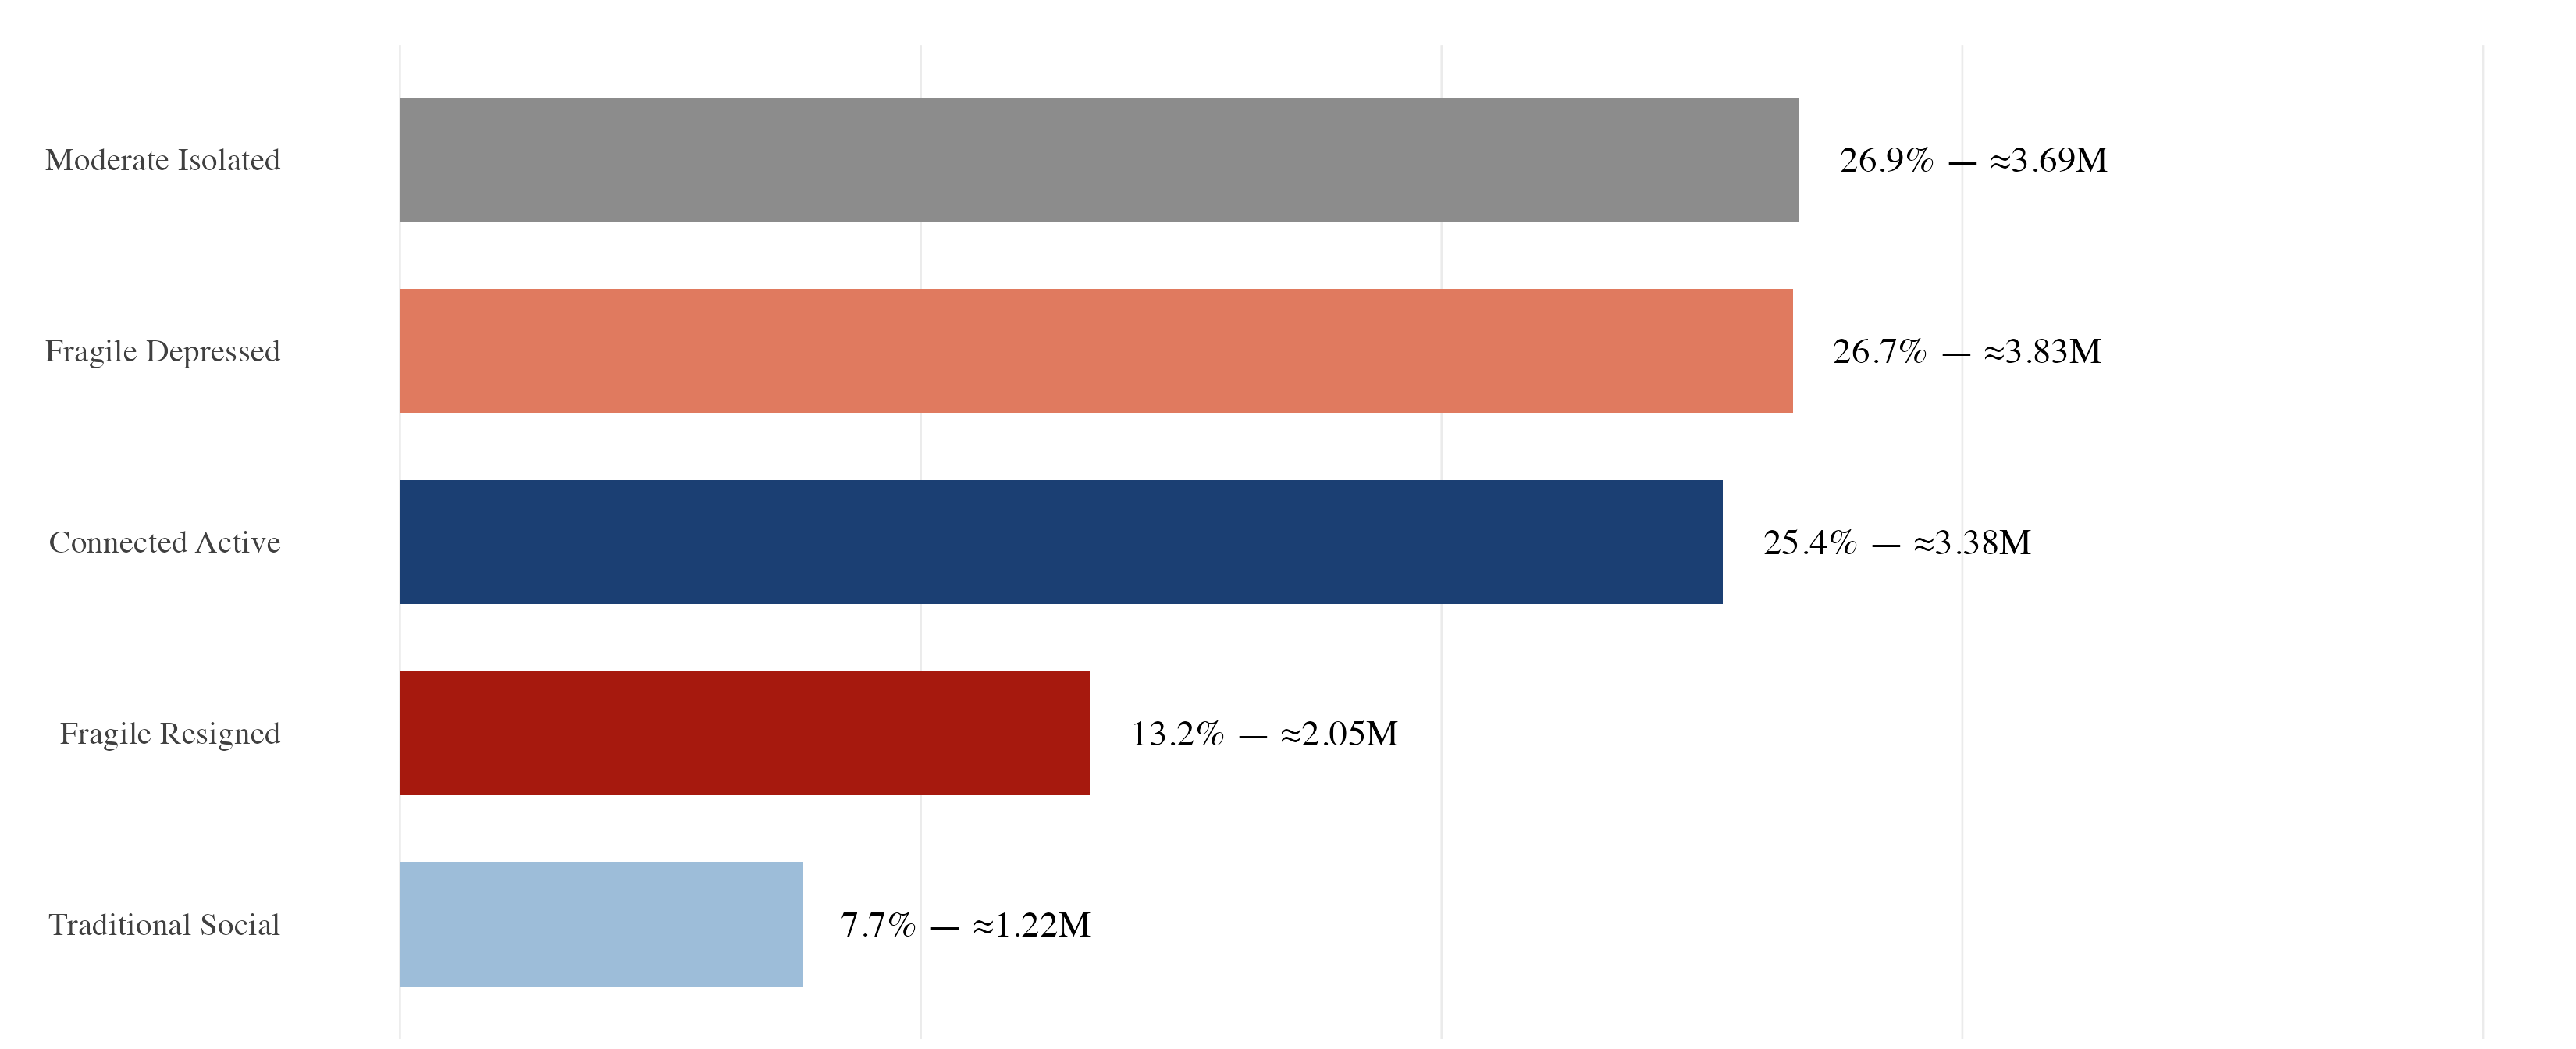
\includegraphics[width=0.95\linewidth]{figures/04_italy/fig_4_8_NEW.png}
  \caption{Population shares of the five Italian archetypes. Bar chart of within-sample shares projected to the Istat 2024 estimate of 14.18 million Italian residents aged 65 or older.}
  \label{fig:ch4-shares}
\end{figure}

